% Figure: Codebase composition
\begin{figure}[t]
\centering
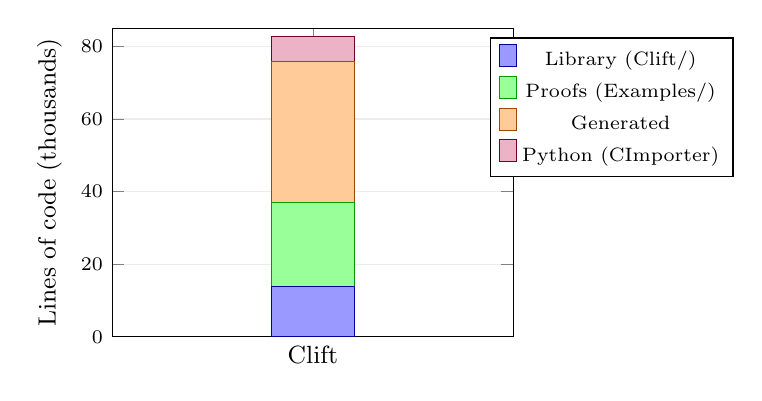
\begin{tikzpicture}
\begin{axis}[
  ybar stacked,
  width=0.55\columnwidth,
  height=5.5cm,
  bar width=30pt,
  ylabel={Lines of code (thousands)},
  ylabel style={font=\small},
  ymin=0, ymax=85,
  xtick=data,
  xticklabels={Clift},
  xticklabel style={font=\small},
  tick label style={font=\scriptsize},
  legend style={font=\scriptsize, at={(1.55,0.97)}, anchor=north east},
  grid=major,
  grid style={gray!15},
  ymajorgrids=true,
  xmajorgrids=false,
]
\addplot[fill=blue!40, draw=blue!60!black] coordinates {(1, 13.9)};
\addplot[fill=green!40, draw=green!60!black] coordinates {(1, 23.0)};
\addplot[fill=orange!40, draw=orange!60!black] coordinates {(1, 39.0)};
\addplot[fill=purple!30, draw=purple!60!black] coordinates {(1, 6.8)};
\legend{Library (Clift/), Proofs (Examples/), Generated, Python (CImporter)}
\end{axis}
\end{tikzpicture}
\caption{Codebase composition by function. Proofs (Examples/) constitute
a large component at 23K LOC. Generated code (39K) dominates---the
CImporter produces extensive L1 bodies, type definitions, and
procedure environments per C file.}
\label{fig:codebase}
\end{figure}
